\appendix
\chapter{Appendix}
If not indicated differently, dimensions and angles specified in the figures
have a tolerance of ±5\%. Unless otherwise noted, all dimensions are in
millimeters (mm). Dimensions and angles defined in the previous chapters may
not be repeated in the figures.

\section{Parking Lot}
\label{fig_parking_lot}
\begin{figure}[H]
	\begin{center}
		\centering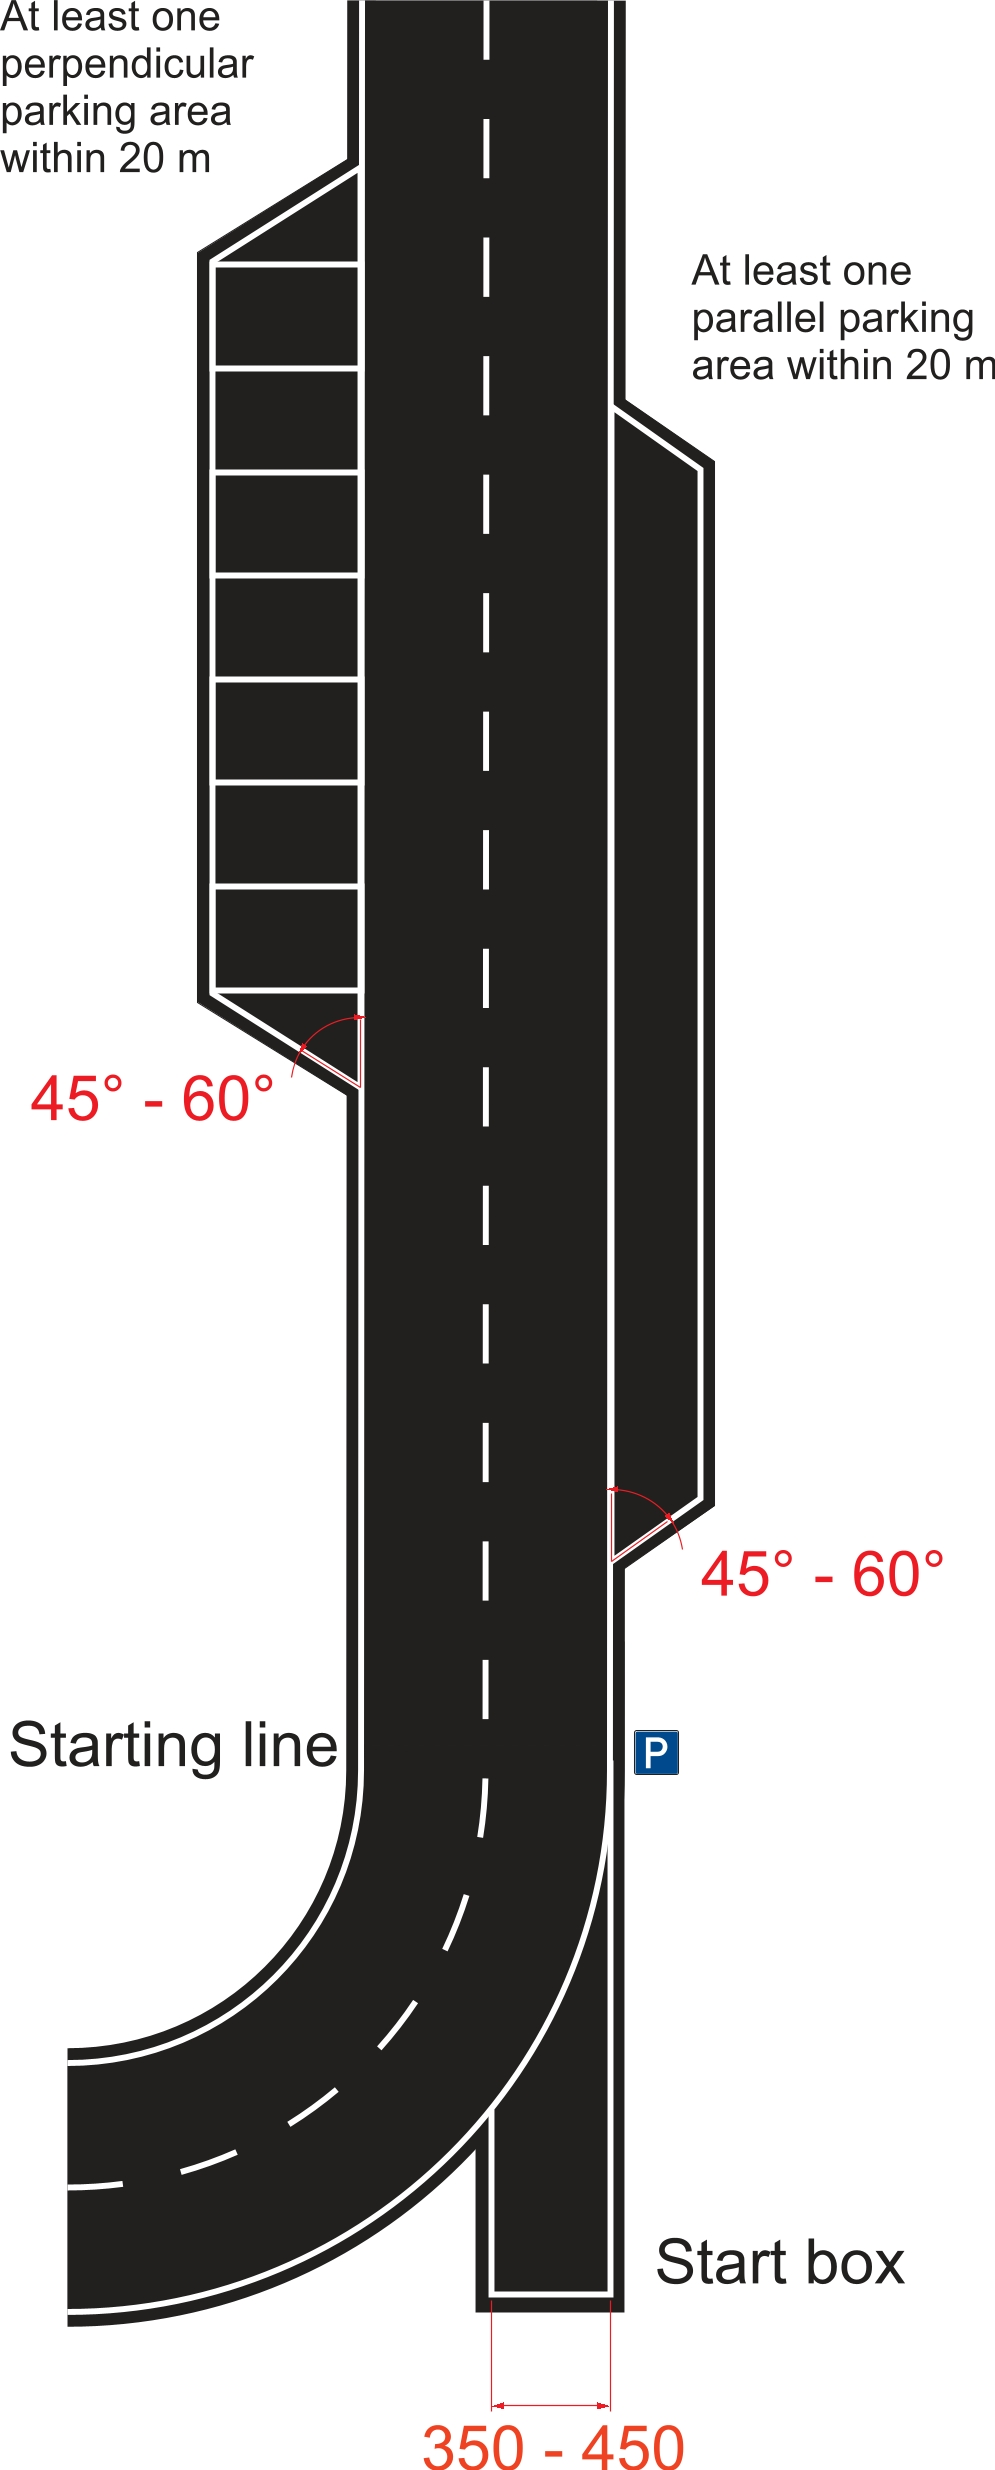
\includegraphics[scale=0.8]{graphics/Abb_1_parking_lot}
	\end{center}
\end{figure}

\section{Parallel Parking}
\label{fig_parallel_parking}
\begin{figure}[H]
	\begin{center}
		\centering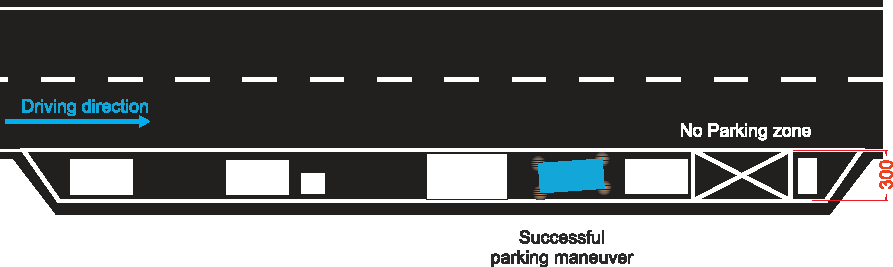
\includegraphics[]{graphics/Abb_2_parallel_parking}
	\end{center}
\end{figure}

\section{Perpendicular Parking}
\begin{figure}[H]
	\label{fig_perpendicular_parking}
	\begin{center}
		\centering\includegraphics[]{graphics/Abb_3_perpendicular_parking}
	\end{center}
\end{figure}

\section{Road Layout and Lane Markings}
\label{fig_road_layout}
\begin{figure}[H]
	\begin{center}
		\centering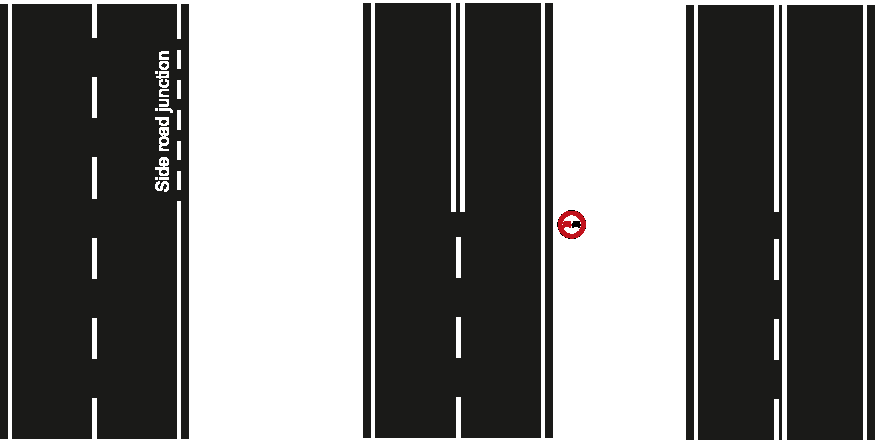
\includegraphics[]{graphics/Abb_4_road_layout}
	\end{center}
\end{figure}

\section{Intersection of the Rural Road Scenario}
\label{fig_intersection_rural}
\begin{figure}[H]
	\begin{center}
		\centering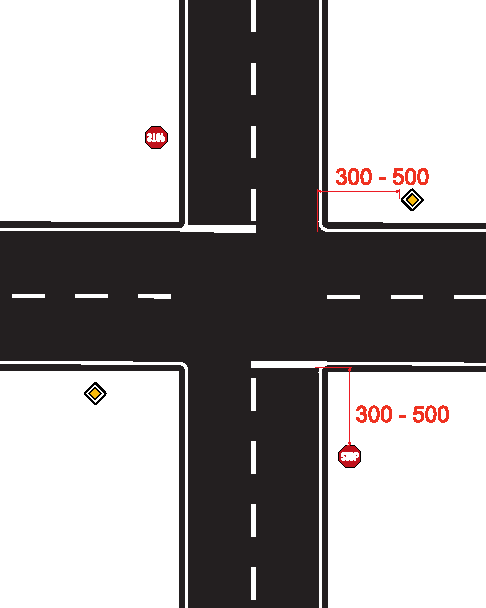
\includegraphics[]{graphics/Abb_5_intersection}
	\end{center}
\end{figure}

\subsection{Dynamic Obstacles at Intersections - Give-Way Condition}
\label{fig_intersection_give_way}
\begin{figure}[H]
	\begin{center}
		\centering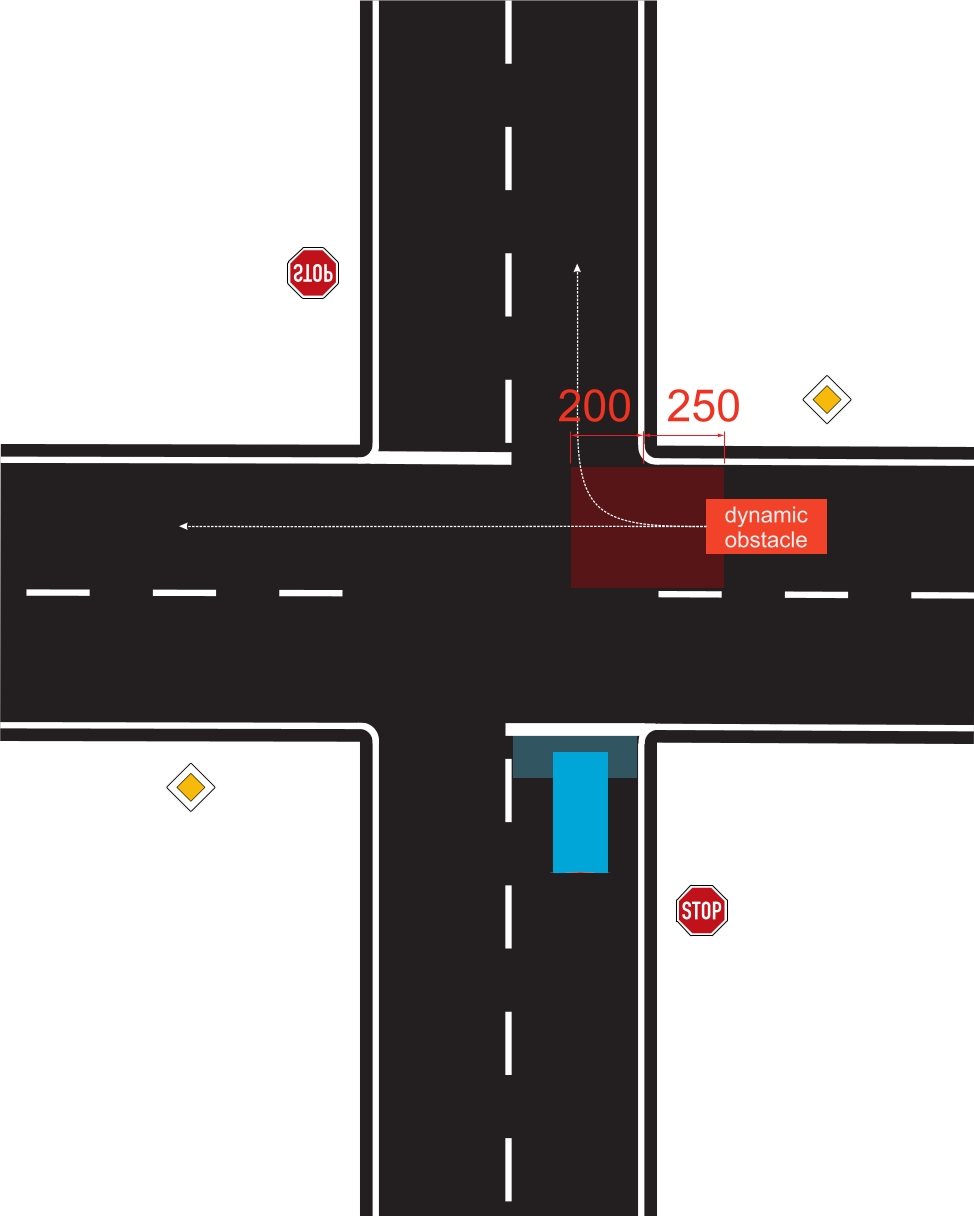
\includegraphics[]{graphics/Abb_6_intersection_give_way}
	\end{center}
\end{figure}

\section{Speed Limit Zone}
\label{fig_speed_limit_zone}
\begin{figure}[H]
	\begin{center}
		\centering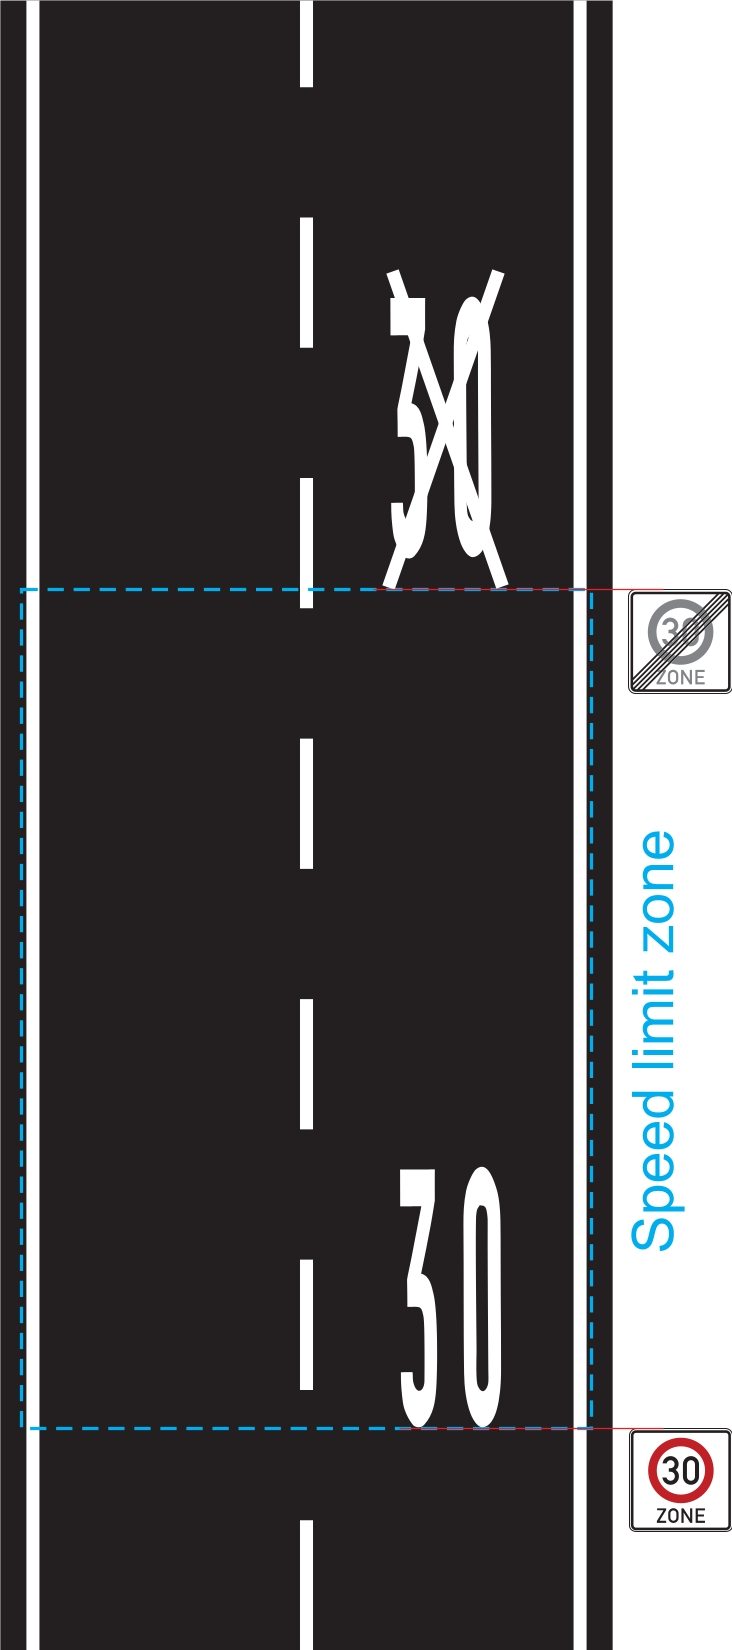
\includegraphics[]{graphics/Abb_7_speed_limit_zone}
	\end{center}
\end{figure}

\section{Barred Area}
\label{fig_barred_area}
\begin{figure}[H]
	\begin{center}
		\centering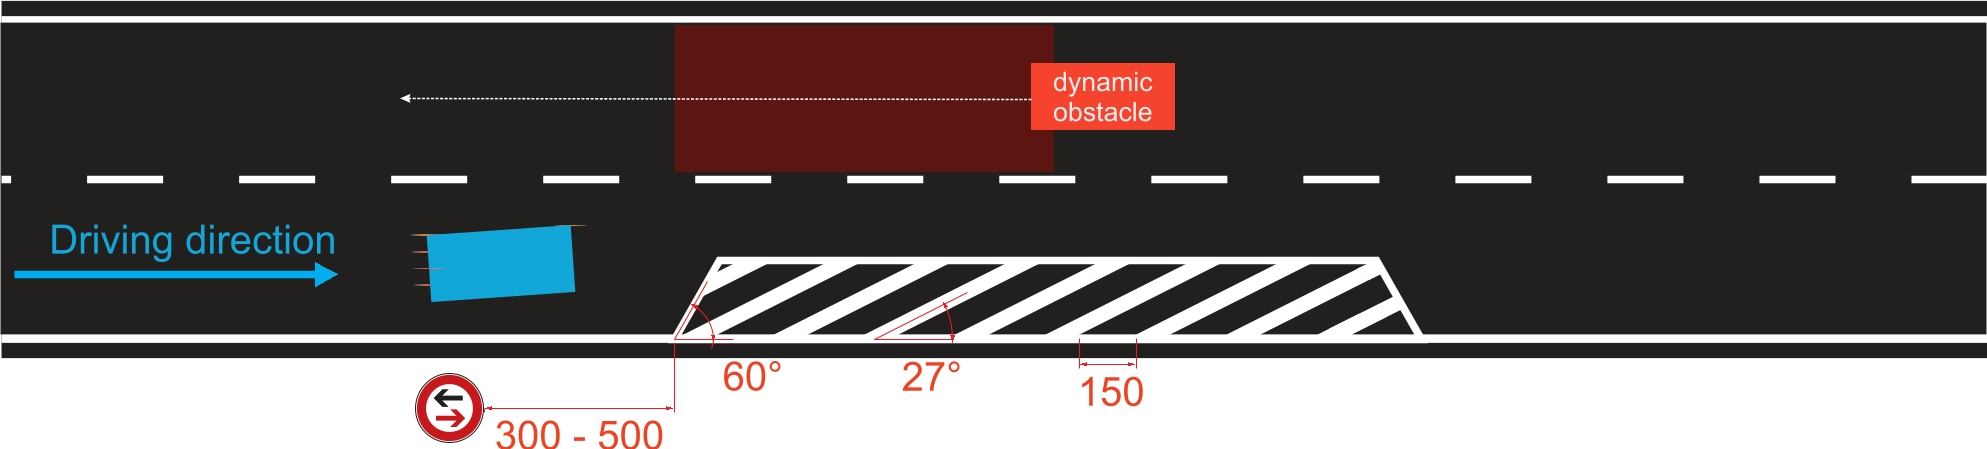
\includegraphics[width=\textwidth]{graphics/Abb_8_barred_area}
	\end{center}
\end{figure}

\section{Crosswalk}
\label{fig_crosswalk}
\begin{figure}[H]
	\begin{center}
		\centering\includegraphics[]{graphics/Abb_9_crosswalk}
	\end{center}
\end{figure}
\newpage

\section{Pedestrian Island}
\colorbox{red}{\large Deprecated}
\begin{figure}[H]
	\begin{center}
		\centering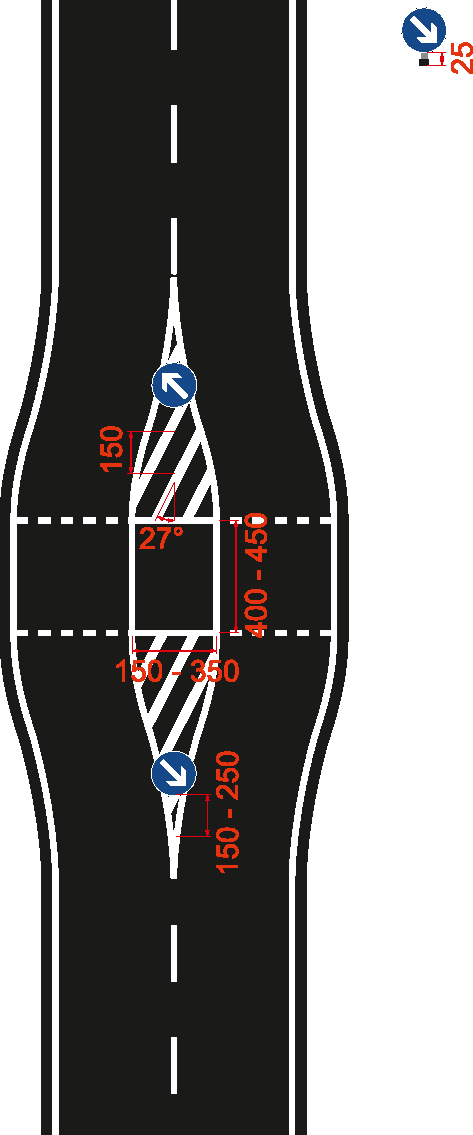
\includegraphics[]{graphics/Abb_10_pedestrian_island}
	\end{center}
\end{figure}
\newpage

\subsection{Pedestrian Island with Crosswalk}
\colorbox{yellow}{\large Deprecated}
\begin{figure}[H]
	\begin{center}
		\centering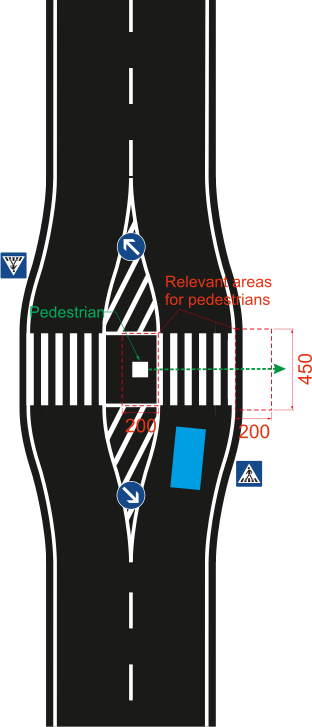
\includegraphics[]{graphics/Abb_11_pedestrian_island_crosswalk}
	\end{center}
\end{figure}

\section{Additional Intersections of the Suburban Scenario}
\label{additional_intersections}

\subsection{Intersection with Give-Way Lines}
\label{fig_intersection_give_way_lines}
\begin{figure}[H]
	\begin{center}
		\centering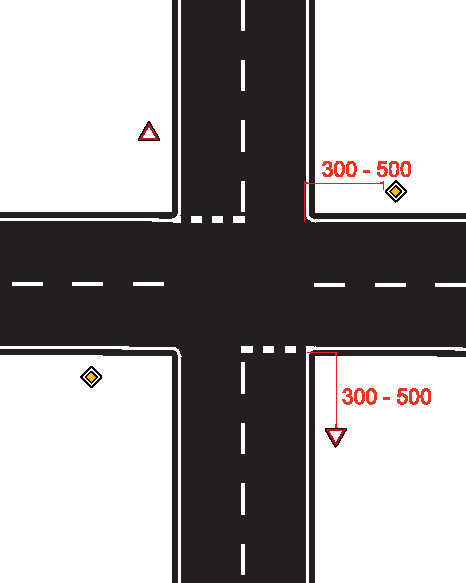
\includegraphics[]{graphics/Abb_12_intersection_give_way_lines}
	\end{center}
\end{figure}

\subsection{Intersection with Priority to Right}
\label{fig_intersection_priority}
\begin{figure}[H]
	\begin{center}
		\centering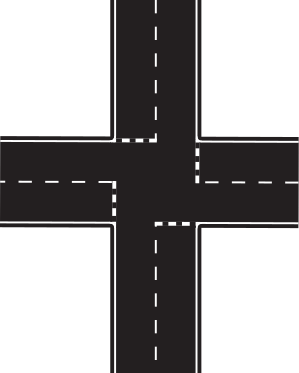
\includegraphics[]{graphics/Abb_13_intersection_priority}
	\end{center}
\end{figure}

\subsection{Intersection with Mandatory Turn}
\label{fig_intersection_mandatory}
\subsubsection{Mandatory Crossing Direction - Stop Condition}
\begin{figure}[H]
	\begin{center}
		\centering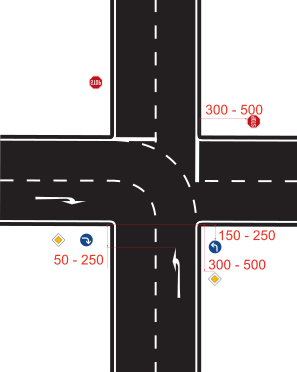
\includegraphics[]{graphics/Abb_14_mandatory_stop}
	\end{center}
\end{figure}

\subsubsection{Mandatory Crossing Direction - Give-Way Condition}
\begin{figure}[H]
	\begin{center}
		\centering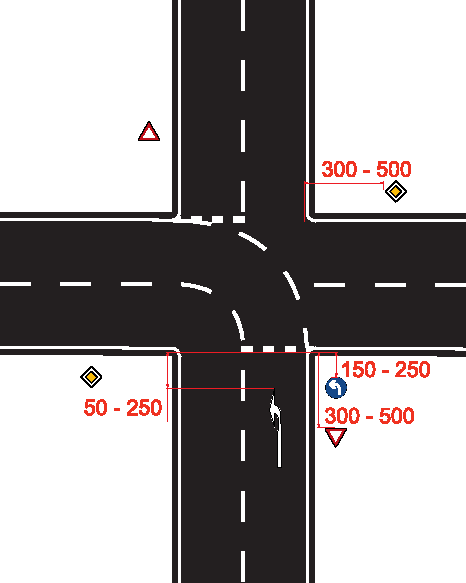
\includegraphics[]{graphics/Abb_15_mandatory_give_way}
	\end{center}
\end{figure}

\subsubsection{Mandatory Crossing Direction - Right of Way Condition}
\begin{figure}[H]
	\begin{center}
		\centering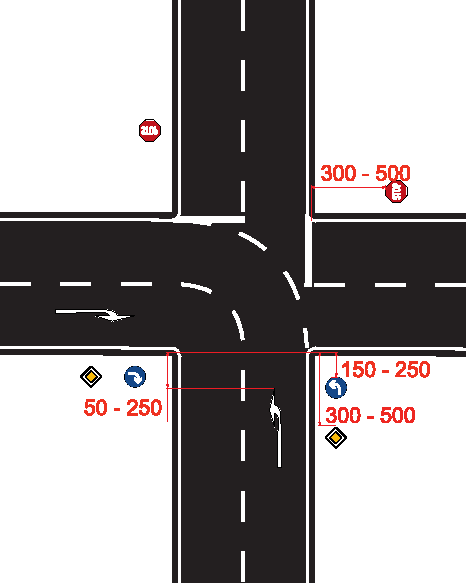
\includegraphics[]{graphics/Abb_16_mandatory_right_of_way}
	\end{center}
\end{figure}

\section{Road Markings}
\label{fig_road_markings}
\begin{figure}[H]
	\begin{center}
		\centering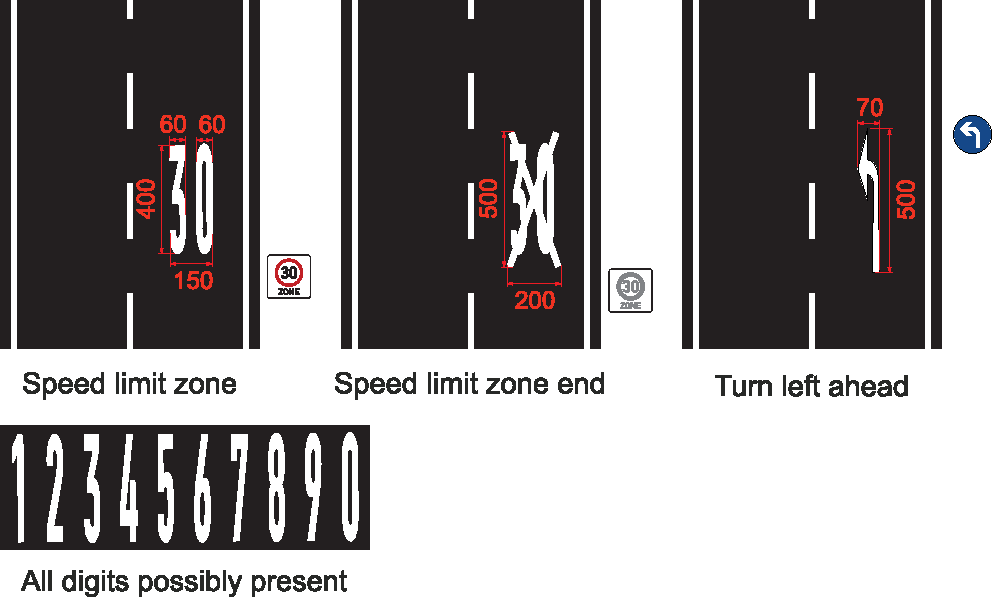
\includegraphics[width=\textwidth]{graphics/Abb_17_road_markings}
	\end{center}
\end{figure}

\section{Traffic Signs}
\label{fig_traffic_signs}
\subsection{Definition of Traffic Signs}
The traffic signs are defined according to StVO (Legal definition of traffic
rules) and are applied as described there, except otherwise defined in this
document. Additional information about the dimensions can be scaled based on
this source.

Traffic signs might appear in their mirrored version as well, e.g. turning
symbols can indicate right or left turns.

\begin{figure}[H]
	\begin{center}
		\centering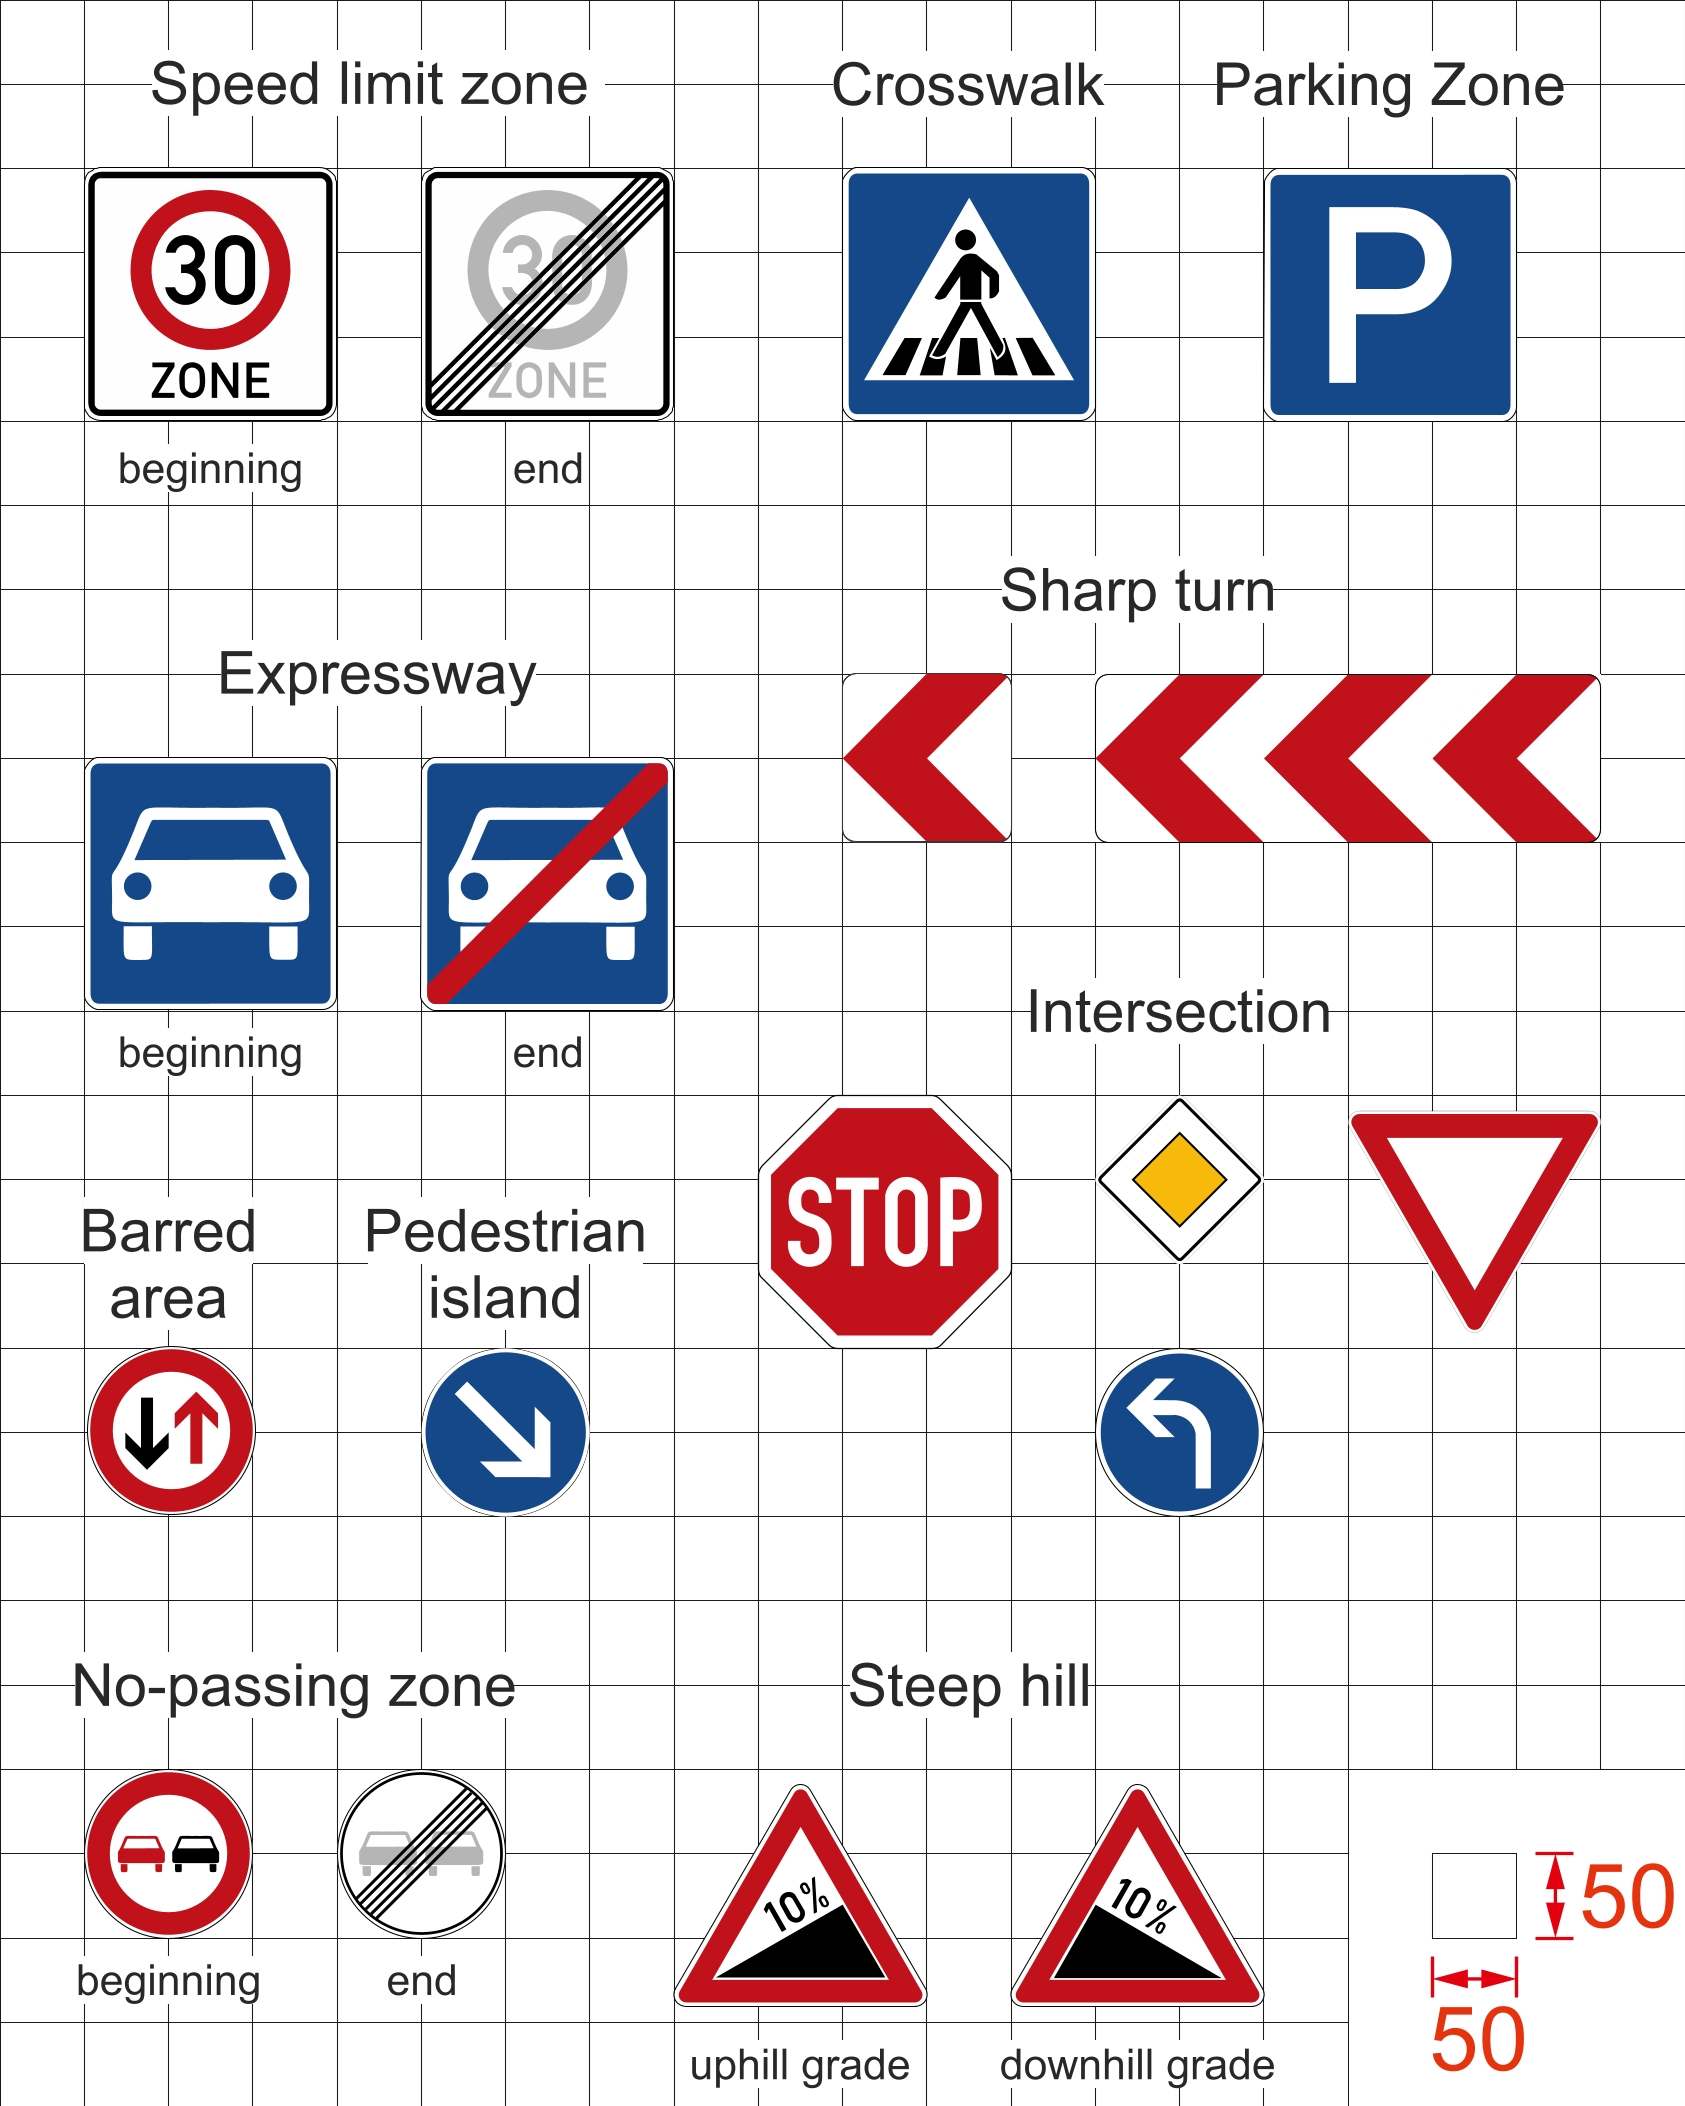
\includegraphics[]{graphics/Abb_18_traffic_signs}
	\end{center}
\end{figure}

\subsection{Positioning of Traffic Signs}
\begin{figure}[H]
	\begin{center}
		\centering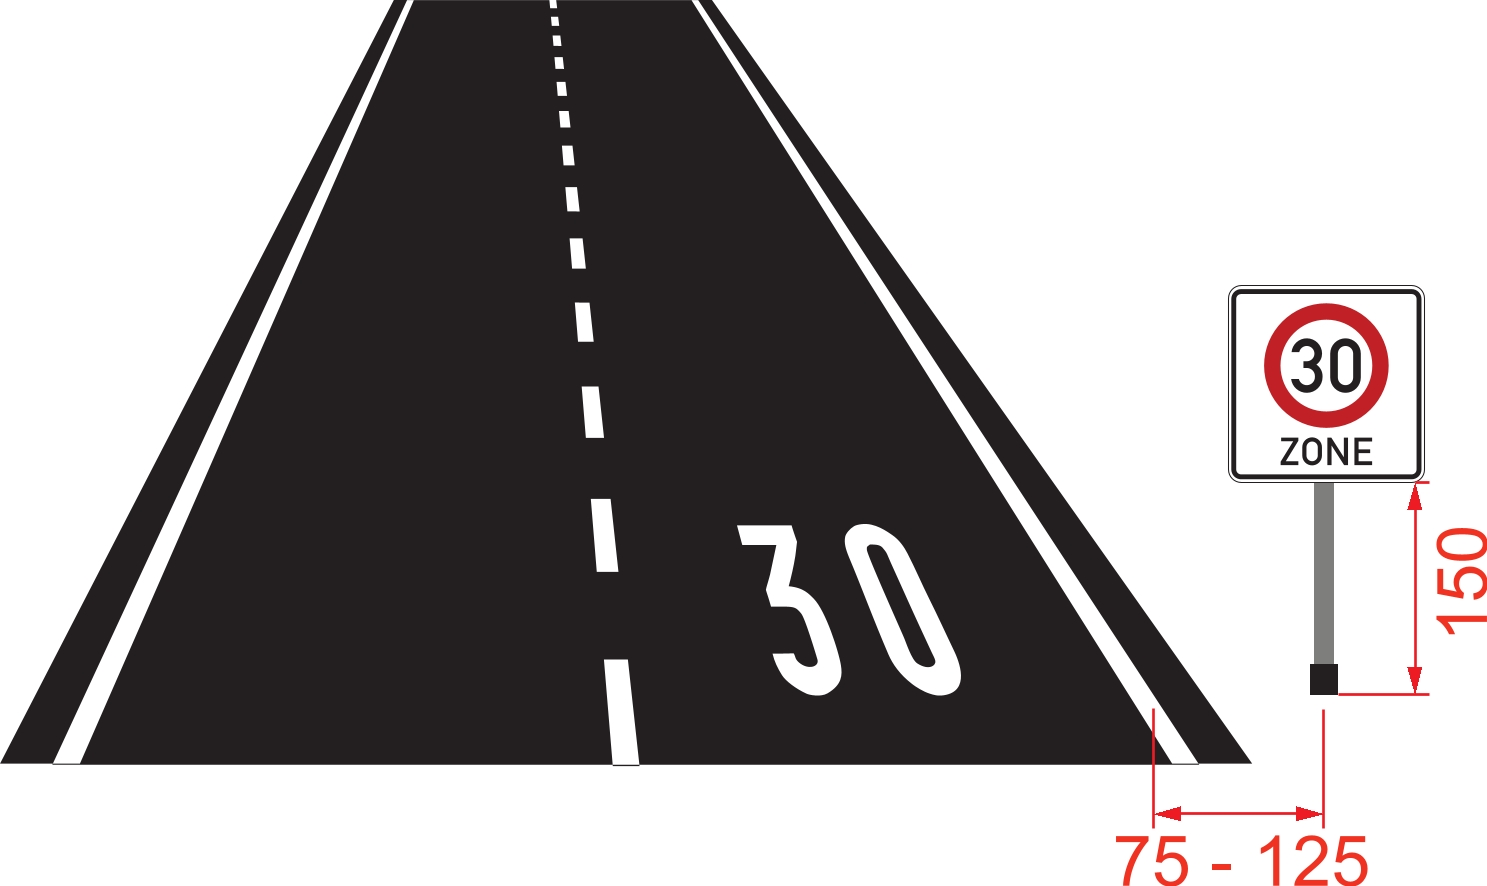
\includegraphics[]{graphics/Abb_19_positioning_of_traffic_signs}
	\end{center}
\end{figure}

\section{Dimensions of Obstacles}
\subsection{Static and Dynamic Obstacles on the Track}
\label{fig_obstacle_dimensions}
\begin{figure}[H]
	\begin{center}
		\centering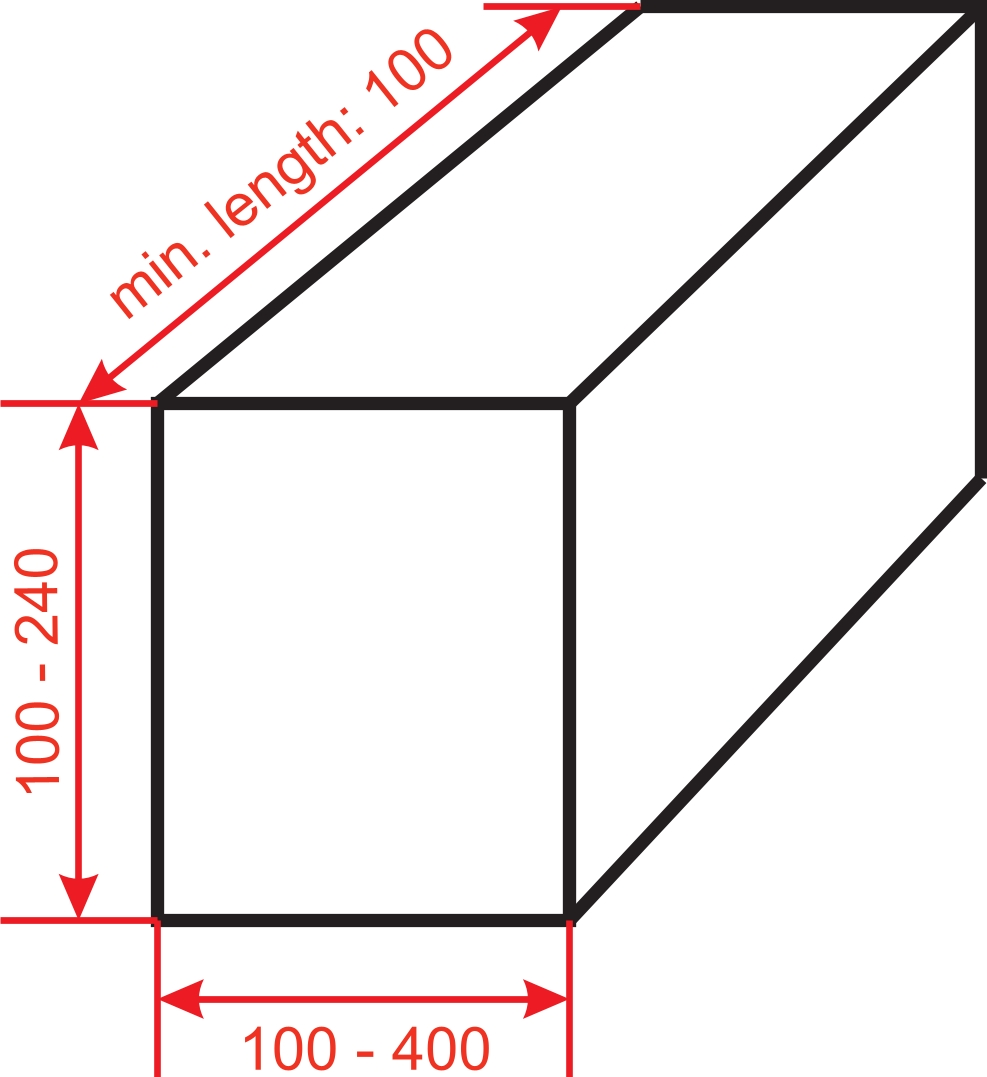
\includegraphics[]{graphics/Abb_20_obstacles}
	\end{center}
\end{figure}

\subsection{Pedestrians}
\label{fig_pedestrians}
\begin{figure}[H]
	\begin{center}
		\centering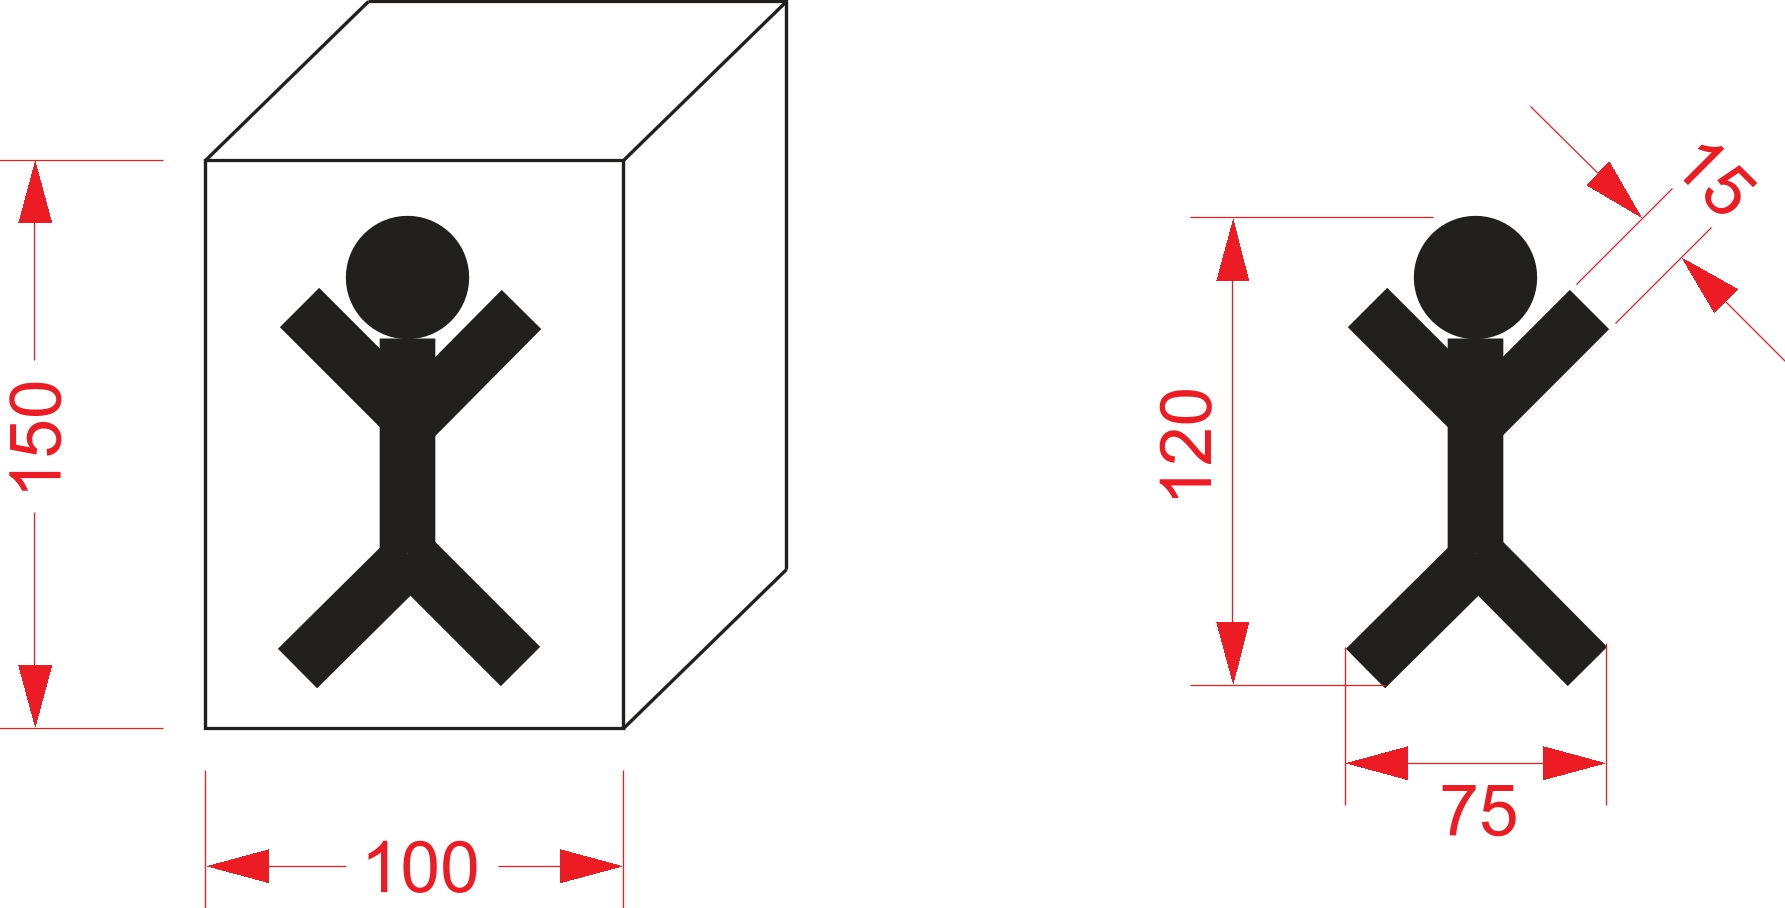
\includegraphics[]{graphics/Abb_21_pedestrians}
	\end{center}
\end{figure}

\section{Example Circuit}
\label{fig_example_circuit}
\vspace*{2cm}
\begin{figure}[H]
	\begin{center}
		\centering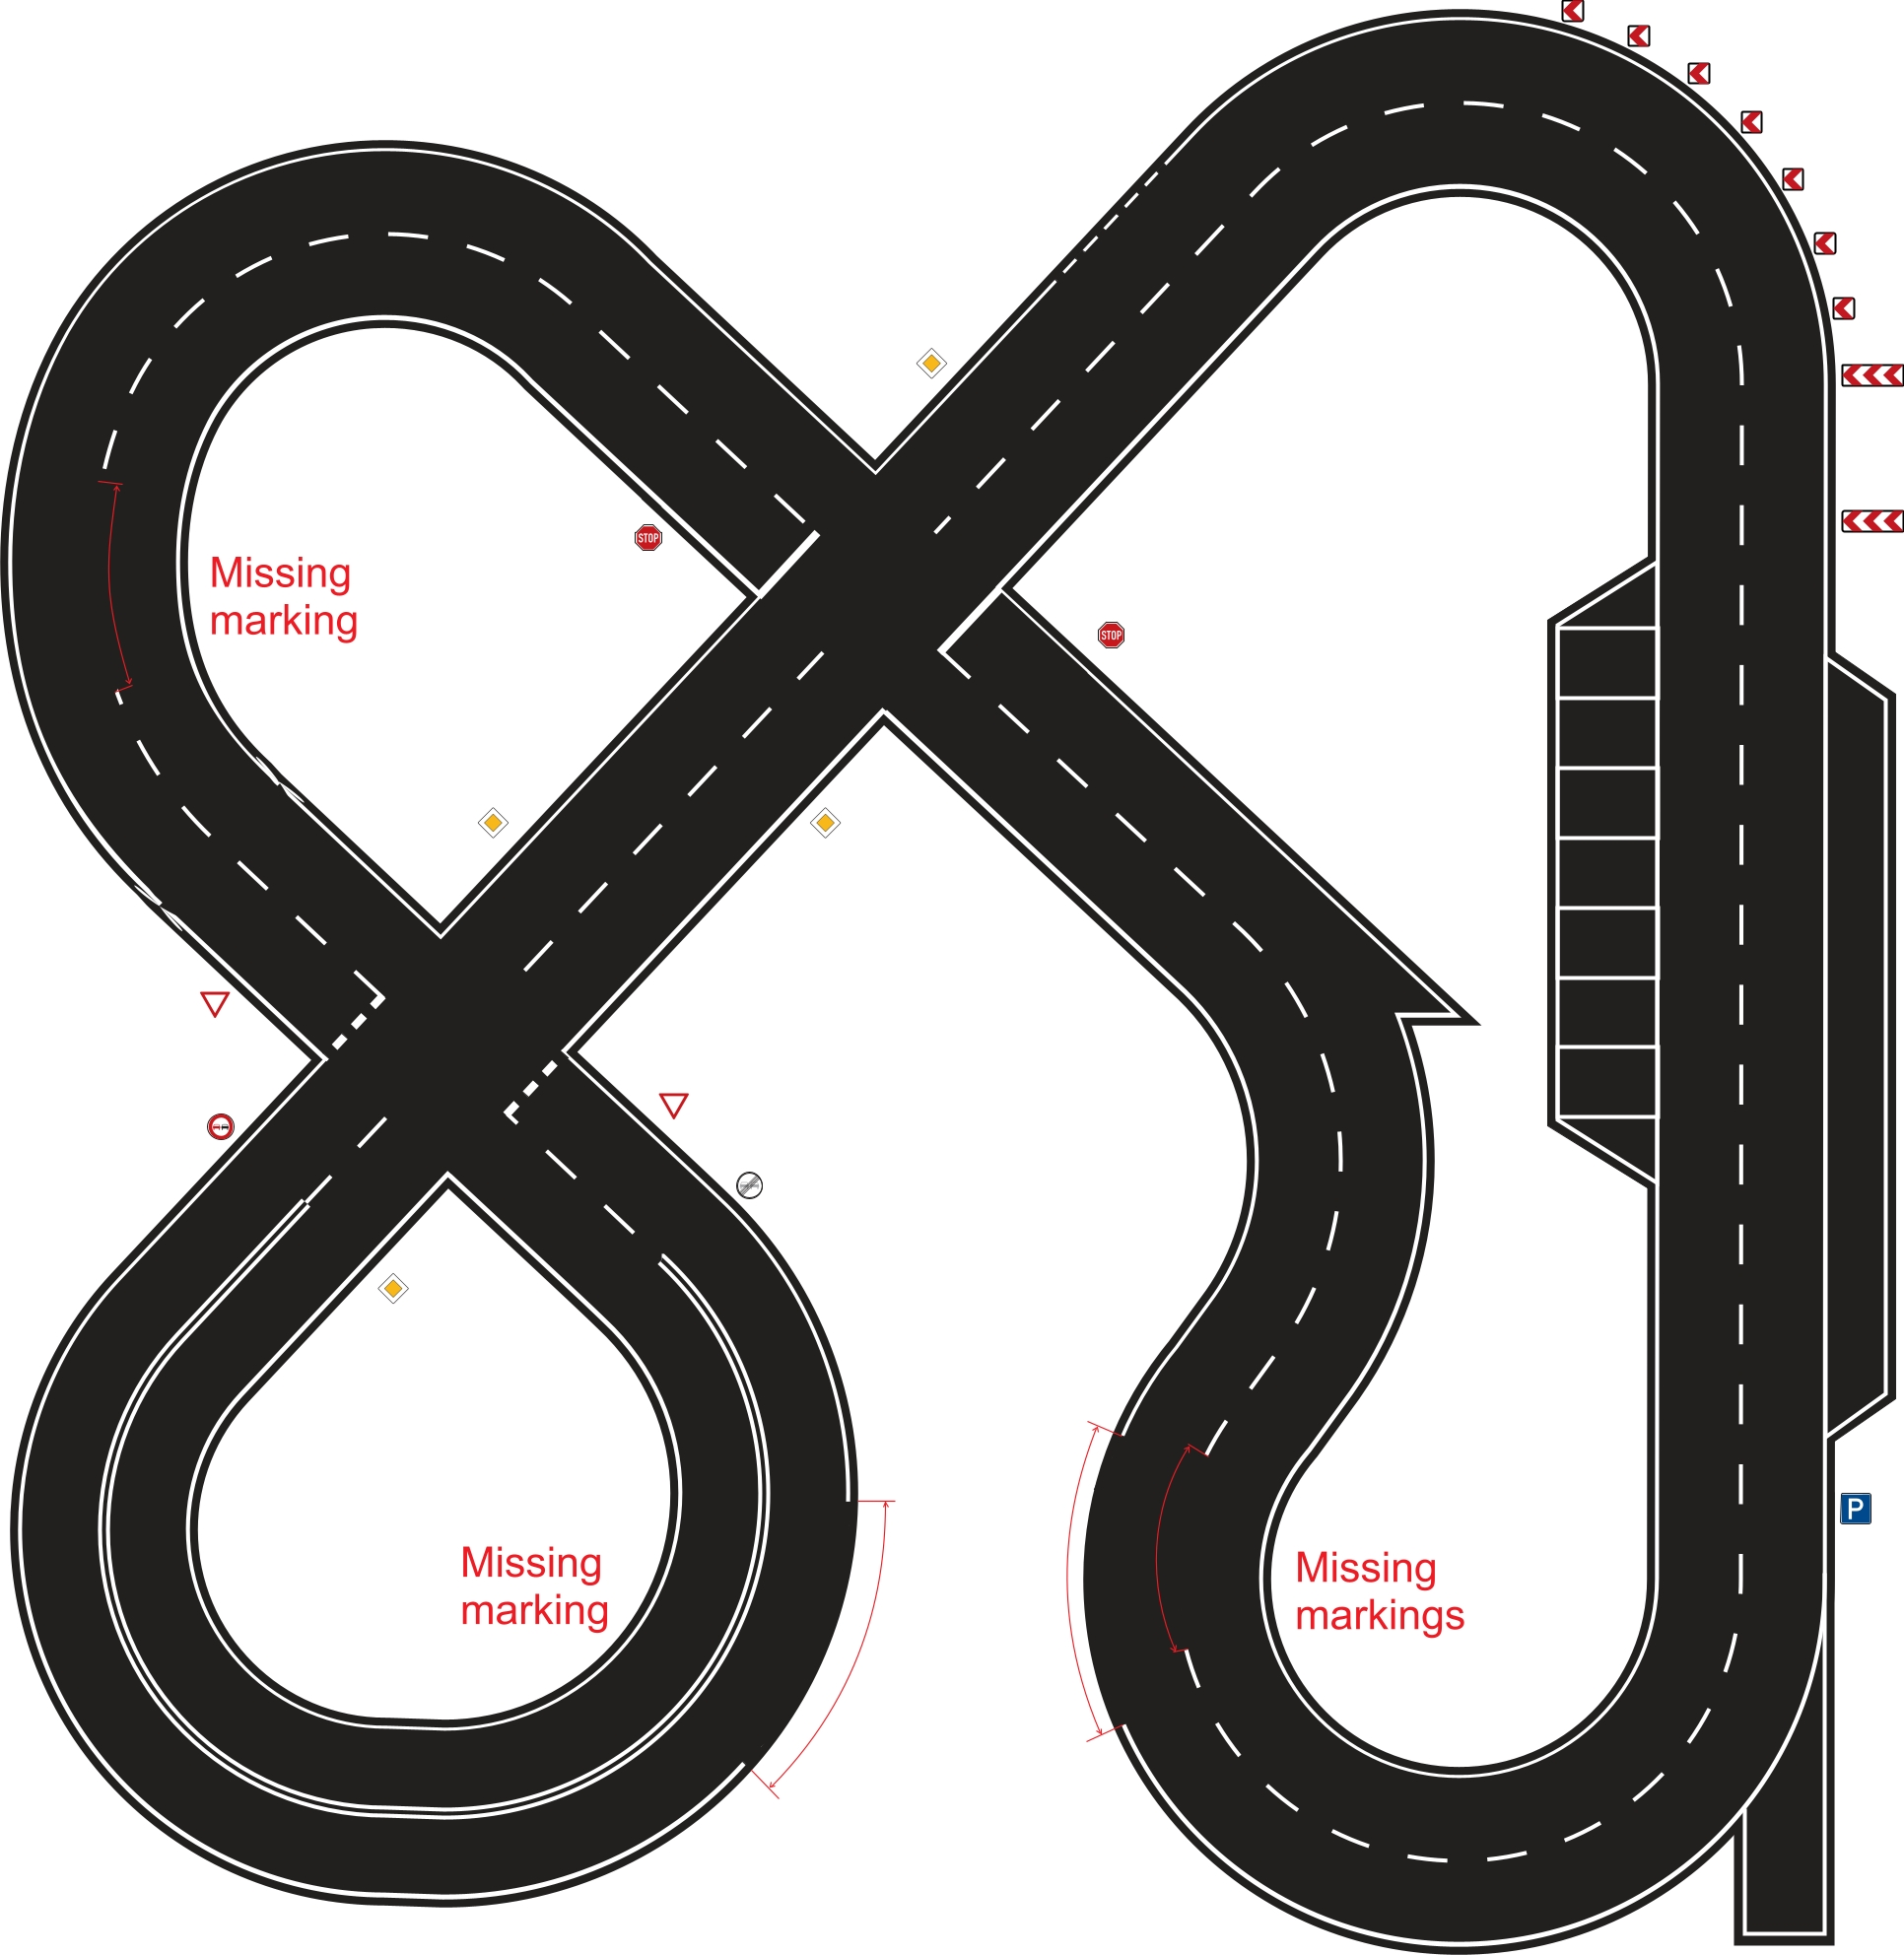
\includegraphics[width=\textwidth]{graphics/Abb_22_example_circuit}
	\end{center}
\end{figure}

\section{Markings of the Start Box Gate}
\label{fig_start_box_markings}
\begin{figure}[H]
	\begin{center}
		\centering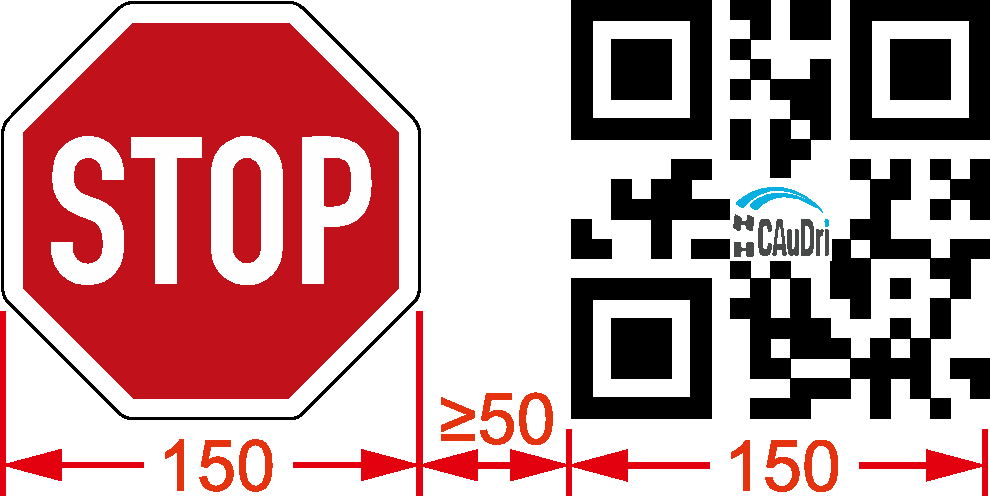
\includegraphics[width=\textwidth]{graphics/Abb_23_start_box_markings}
	\end{center}
\end{figure}